% ------------------------ LaTeX Project Note Template ------------------------

% -- Set document class and font size ---
\documentclass[a4paper, 11pt]{article}

% -- Package imports --------------------
\usepackage[dvipsnames]{xcolor}
\usepackage{
    amsmath, amsthm, amssymb, mathtools, dsfont, units, physics,
    graphicx, wrapfig, float, booktabs, changepage,
    listings, inconsolata, pythonhighlight, subcaption,
    fancyhdr, hyperref, enumerate, enumitem, float }

% Load minted separately -- requires -shell-escape
\usepackage[most, minted]{tcolorbox}

% -- Page layout settings ---------------

% Set page margins
\usepackage[margin=3cm, a4paper, footskip=12mm]{geometry}

% Anchor footnotes to the bottom of the page
\usepackage[bottom]{footmisc}

% Set line spacing
\renewcommand{\baselinestretch}{1.2}

% Set spacing between paragraphs
\setlength{\parskip}{1.3mm}

% Allow multi-line equations to break onto the next page
\allowdisplaybreaks

% Get rid of paragraph indentation
\setlength{\parindent}{0pt}


% -- Page formatting settings -----------

% Set image captions to be italicized
\usepackage[font={it,footnotesize}]{caption}

% Set link colors for labeled items (blue), citations (red), URLs (orange)
\hypersetup{colorlinks=true, 
    linkcolor=RoyalBlue, 
    citecolor=RedOrange,
    urlcolor=ForestGreen
}

% Set font size for section titles (\large) and subtitles (\normalsize)
\usepackage{titlesec}
\titleformat{\section}{\Large\bfseries}{{\fontsize{19}{19}\selectfont\textreferencemark}\;\; }{0em}{}
\titleformat{\subsection}{\large\bfseries\selectfont}{\thesubsection\;\;\;}{0em}{}

% -- Table of Contents settings ---------
\usepackage[subfigure]{tocloft}

% Reduce spacing between sections in table of contents
\setlength{\cftbeforesecskip}{0.9ex}
\cftsetindents{section}{0em}{0em}
\renewcommand{\cfttoctitlefont}{\Large\bfseries}

% SAFE WAY: Remove section numbering width constraints in TOC 
% instead of opening unclosed \lrbox structures
\setcounter{tocdepth}{3} 
\renewcommand{\cftsecnumwidth}{0pt} 
\renewcommand{\cftsecindent}{0pt}

% -- Set path for images ----------------
\graphicspath{{figures/}{../figures/}}

% -- Math/Statistics commands -----------

% Add a reference number to a single line of a multi-line equation.
% Usage: "\numberthis\label{labelNameHere}" in an align or gather environment.
\newcommand\numberthis{\addtocounter{equation}{1}\tag{\theequation}}

% Set up Tikz for diagrams
\usepackage{tikz}
\usepackage{tikz-cd}
\usetikzlibrary{intersections, angles, quotes, calc, positioning}
\usetikzlibrary{arrows.meta}
\usepackage{pgfplots}
\pgfplotsset{compat=1.13}

\tikzset{
    force/.style={thick, {Circle[length=2pt]}-stealth, shorten <=-1pt}
}

% Set up different styles for theorems/remarks/notes/proofs/etc.
\usepackage{thmtools}
\usepackage[framemethod=TikZ]{mdframed}
\mdfsetup{skipabove=1em,skipbelow=0em}


\theoremstyle{definition}

\declaretheoremstyle[
    headfont=\bfseries\sffamily\color{ForestGreen!70!black}, bodyfont=\normalfont,
    mdframed={
        linewidth=2pt,
        rightline=false, topline=false, bottomline=false,
        linecolor=ForestGreen, backgroundcolor=ForestGreen!5,
    }
]{thmgreenbox}

\declaretheoremstyle[
    headfont=\bfseries\sffamily\color{NavyBlue!70!black}, bodyfont=\normalfont,
    mdframed={
        linewidth=2pt,
        rightline=false, topline=false, bottomline=false,
        linecolor=NavyBlue, backgroundcolor=NavyBlue!5,
    }
]{thmbluebox}

\declaretheoremstyle[
    headfont=\bfseries\sffamily\color{NavyBlue!70!black}, bodyfont=\normalfont,
    mdframed={
        linewidth=2pt,
        rightline=false, topline=false, bottomline=false,
        linecolor=NavyBlue
    }
]{thmblueline}

\declaretheoremstyle[
    headfont=\bfseries\sffamily\color{RawSienna!70!black}, bodyfont=\normalfont,
    mdframed={
        linewidth=2pt,
        rightline=false, topline=false, bottomline=false,
        linecolor=RawSienna, backgroundcolor=RawSienna!5,
    }
]{thmredbox}

\declaretheoremstyle[
    headfont=\bfseries\sffamily\color{RawSienna!70!black}, bodyfont=\normalfont,
    numbered=no,
    mdframed={
        linewidth=2pt,
        rightline=false, topline=false, bottomline=false,
        linecolor=RawSienna, backgroundcolor=RawSienna!1,
    },
    qed=\qedsymbol
]{thmproofbox}

\declaretheoremstyle[
    headfont=\bfseries\sffamily\color{NavyBlue!70!black}, bodyfont=\normalfont,
    numbered=no,
    mdframed={
        linewidth=2pt,
        rightline=false, topline=false, bottomline=false,
        linecolor=NavyBlue, backgroundcolor=NavyBlue!1,
    },
]{thmexplanationbox}

\declaretheorem[style=thmgreenbox, name=Key Idea]{definition}
\declaretheorem[style=thmbluebox, numbered=no, name=Example]{eg}
\declaretheorem[style=thmredbox, name=Claim]{prop}
\declaretheorem[style=thmredbox, name=Theorem]{theorem}

\declaretheorem[style=thmproofbox, name=Proof]{replacementproof}
% FIXED: Braces are now perfectly balanced
\renewenvironment{proof}[1][\proofname]{\vspace{-10pt}\begin{replacementproof}}{\end{replacementproof}}

\declaretheorem[style=thmexplanationbox, name=Explanation]{tmpexplanation}
\newenvironment{explanation}[1][]{\vspace{-10pt}\begin{tmpexplanation}}{\end{tmpexplanation}}


\declaretheorem[style=thmbluebox, numbered=no, name=Remark]{remark}
\declaretheorem[style=thmbluebox, numbered=no, name=Note]{note}

\newtheorem*{notation}{Notation}
\newtheorem*{previouslyseen}{As previously seen}
\newtheorem*{problem}{Problem}
\newtheorem*{observe}{Observe}
\newtheorem*{property}{Property}
\newtheorem*{intuition}{Intuition}

\newtcblisting{cppcode}{
    listing engine=minted,
    minted language=cpp,
    minted style=friendly,
    minted options={fontsize=\small, breaklines, autogobble},
    colback=gray!20,
    colframe=black,
    listing only,
    left=4mm,
    top=1mm,
    bottom=1mm,
}

\newtcblisting{bashcode}{
    listing engine=minted,
    minted language=bash,
    minted style=friendly,
    minted options={fontsize=\small, breaklines, autogobble},
    colback=gray!20,
    colframe=black,
    listing only,
    left=1mm,
    top=1mm,
    bottom=1mm,
}

\newtcblisting{tomlcode}{
    listing engine=minted,
    minted language=toml,
    minted style=friendly,
    minted options={fontsize=\small, breaklines, autogobble},
    colback=gray!20,
    colframe=black,
    listing only,
    left=4mm,
    top=1mm,
    bottom=1mm,
}

\newtcblisting{pythoncode}{
    listing engine=minted,
    minted language=python,
    minted style=friendly,
    minted options={fontsize=\small, breaklines, autogobble},
    colback=gray!20,
    colframe=black,
    listing only,
    left=4mm,
    top=1mm,
    bottom=1mm,
}


\newtcblisting{inputdeck}{
    listing engine=minted,
    minted language=text,
    minted style=friendly,
    minted options={fontsize=\small, breaklines, autogobble},
    colback=gray!20,
    colframe=black,
    listing only,
    left=4mm,
    top=1mm,
    bottom=1mm,
}

% -- Left/right header text -------------
\usepackage{fancyhdr}
\pagestyle{fancy}
\fancyhf{} % Explicitly reset everything safely

\setlength{\headheight}{15pt}
\renewcommand{\footrulewidth}{0pt}
\renewcommand{\headrulewidth}{0.4pt}

% Use the native automated marking engine safely
\renewcommand{\sectionmark}[1]{\markright{#1}}

\fancyhead[R]{\small\textit{\nouppercase{\rightmark}}}
\fancyfoot[C]{\thepage}
\date{}

% Left header text: short title, hyperlinked to table of contents. Can't put 
% this in the preamble as it changes per document.
%\fancyhead[L]{\hyperref[sec:contents]{\small Photon Kinetics in OSIRIS -- 
%Master Document}}

\begin{document}

% -- Main title and subtitle ---------------
\title{Photon Kinetics in OSIRIS -- Master Document\vspace{-2.5em}}

% -- Add title and table of contents -------
\maketitle
\thispagestyle{empty}

\begin{adjustwidth}{15mm}{18mm}
\hspace{1.4em} This document serves as a technical reference for FP-Tools, a
molecular dynamics trajectory analysis code developed at Los Alamos National
Laboratory. It covers the physical background behind each implemented analysis, 
the details of the C++ implementation, build and usage instructions, and notes
on design decisions made throughout development. It is intended both for users
who want to run the code and developers who want to understand, modify, or
extend it.

\hspace{1.4em}\textit{Disclaimer:} This document will inevitably contain some 
mistakes ---  both simple typos and legitimate errors, so take what you read
with a grain of salt. If you find mistakes and feel like telling me, I would be
grateful and happy to hear from you, even for the most trivial of errors. You 
can reach me by email at \href{mailto:lghart@umich.edu}{lghart@umich.edu}.
\end{adjustwidth}
\vspace{10.5cm}
\begin{center}
        \textit{You can find more notes like this on my website \href{https://leahghartman.github.io/academics/}{here}}
        \rule{0.75\textwidth}{0.5pt} \\
        Leah Hartman \\
        \date{\normalsize Last updated: \today} \\
        University of Michigan Applied Physics
\end{center}

\newpage
\tableofcontents\label{sec:contents}

% -- Main content: import subfiles ---------
\newpage
\section{Introduction}
This section will cover the theoretical background for this project.


\subsection{Motivation and Scope}
\subsection{Notation and Normalized Units}
\subsection{Document Roadmap}



\newpage
\section{Theoretical Background}

\subsection{Laser-Plasma Interactions: Overview}
\subsection{The Ponderomotive Force}

\subsection{Plasma Wakefields}
\subsubsection{Linear Regime}
\subsubsection{Nonlinear Regime}

\subsection{Photon Kinetics as a Concept}
\subsubsection{Equations of Motion}
\subsubsection{Coupling to the Plasma}

\subsection{Comparison to the Full EM Treatment}




\newpage
\section{Numerical Methods}

This section describes the numerical methods used in the photon kinetics
module in OSIRIS. It begins with how the photons are advanced (Time Integration),
how photon and electron densities are deposited onto the grid (Density
Deposition), how their gradients are calculated (Gradient Deposition), how
the grid quantities are filtered (Smoothing and Filtering), and conventions
for the units. This section assumes that you've read the Theoretical Background 
section, which contains the equations of motion that will be discretized here.
To see the  code that is actually implemented, see the OSIRIS Implementation 
section.

\subsection{Time Integration}

Here we will cover....

\subsubsection{Discretizing the Equations of Motion}

The ray equations are derived in the Theoretical Background section and are only
restated here. In OSIRIS units (lengths normalized by $c/\omega_{p0}$, times
normalized by $1/\omega_{p0}$, density normalized by $n_0$), a photon 
macro-particle with position $\mathbf{x}$ and wavenumber $\mathbf{k}$ obeys
\begin{equation*}
    \frac{d\mathbf{x}}{dt} = \frac{\mathbf{k}}{\omega}\,,
    \qquad
    \frac{d\mathbf{k}}{dt} = -\frac{1}{2\,\omega}\nabla n_e\,,
    \qquad
    \omega = \sqrt{|\mathbf{k}|^{2} + n_e(\mathbf{x})}\,.
    \label{eq:ray_equations}
\end{equation*}

\paragraph{What has to be discretized.}
Time is advanced in  ...

\paragraph{What the integrator should do.} We ultimately care about how this
code performs for the application of photon acceleration, in which the quantity
we care about is the wavenumber, $\mathbf{k}$. Any kind of numerical drift in
$\mathbf{k}$ will therefore appear as an unphysical frequency drift. The 
integrator should:
\begin{enumerate}

    \item \textbf{Not let $\omega$ drift.} In a stationary medium, $\omega$ is
    exactly conserved, ...

    \item \textbf{Be second order accurate.} We'd like to match the accuracy of
    the rest of the OSIRIS code, so this rules out integrators like RK4.

    \item \textbf{Use as little gathers as possible.} This is basically expensive

\end{enumerate}
The comparison across the next few sections evaluates how each integration 
scheme meets the above requirements.

\subsubsection{Naive Leapfrog Implementation}
We start from a Hamiltonian which is separated into a kinetic part that depends
only on momentum and a potential part that depends only on position: 
$H(\mathbf{q}, \mathbf{p}) = T(\mathbf{p}) + V(\mathbf{x})$.

In the above cases where the Hamiltonian is separable, the equations of motion
are given by
\begin{align*}
    \dot{\mathbf{q}} &= \nabla_{\mathbf{p}} \, H(\mathbf{q}, \mathbf{p}) = \nabla_
    {\mathbf{p}} \, T(\mathbf{p}), \\
    \dot{\mathbf{p}} &= -\nabla_{\mathbf{q}} \, H(\mathbf{q}, \mathbf{p}) = -\nabla_
    {\mathbf{q}} \, V(\mathbf{q}). 
\end{align*}
Each piece can be integrated exactly on its own: a solution for the coordinates
can be found if the momenta are kept constant and vice versa. These solutions 
can be combined in a time-symmetric fashion to give you the leapfrog method. There
are a few different types:
\begin{itemize}

    \item \textbf{Staggered Leapfrog.} This is the standard in PIC codes and what
    I'll be referring to from this point forward. This framing updates the
    position and velocity at interleaved times.

    \item \textbf{Velocity Verlet/Position Verlet.} These are mathematically
    equivalent to staggered Leapfrog, but synchronizes positions and velocities
    to the same integer timesteps. The difference between the velocity or
    position Verlet algorithms is simply the order of the updates.

    \item \textbf{Central-Difference Leapfrog.}

\end{itemize}

Leapfrog is the standard in PIC codes for a few reasons:
\begin{enumerate}

    \item \textbf{Time-reversible:} if you advance the solution from some
    initial condition to a future point, you can then make that point your new
    initial condition and step back to where you started.

    \item \textbf{Symplectic:} preserves the phase-space area/volumn (in 
    canonical units).

    \item \textbf{Explicit:} calculates a future state directly with the 
    current available information, at the cost of being conditionally stable
    and requiring smaller timesteps.

\end{enumerate}

\paragraph{Why leapfrog won't work for this case.} The Hamiltonian for a 
photon in this situation is $H = \omega = \sqrt{k^2 + n_e(x)}$, which isn't 
separable. $\omega$ depends on both $x$ and $k$, so neither $\dot{x} = k/\omega$
or $\dot{k} = -(1/2\omega)\nabla n_e$ can be written as a function of one 
variable alone. Because leapfrog isn't even well-defined or applicable in its
usual form this way, we look for other integrators.

You can see the consequences of this in the following single-photon test

\subsubsection{The Predictor-Corrector Method}
\paragraph{Why not a symplectic or implicit method?} A simple way to keep the
symplectic property for a non-separable Hamiltonian (while also maintaining only
second-order accuracy) is the lowest-order symplectic Runge-Kutta method. 
To turn RK2 symplectic, one can use ...., which as a side effect also makes the
integrator implicit (the implicit midpoint rule):

EQN HERE

\paragraph{The scheme.} The scheme chosen for the photon kinetic module is an 
explicit trapezoidal predictor-corrector method (Heun's method). In general, 
these update equations are given by:


\subsubsection{Accuracy and Stability}


\subsection{Density Deposition}


\subsection{Gradient Deposition}
\subsubsection{Old Method: Direct Gradient Gather}
\subsubsection{New Method: Deposit-then-Gather}
\subsubsection{Sign Convention and Equivalence}


\subsection{Smoothing and Filtering}
\subsection{Normalization and Units}


\newpage
\section{OSIRIS Implementation}

\subsection{Code Architecture Overview}
    \subsubsection{Key Files and Modules}
    \subsubsection{Data Flow per Timestep}


\subsection{1D Cartesian Implementation}
    \subsubsection{advance\_deposit\_pkt}
    \subsubsection{advance\_photons\_1d}
    \subsubsection{dudt\_boris\_feedback\_pkt}

\subsection{2D Cartesian Implementation}



\subsection{Quasi-3D / Cylindrical Implementation}
    \subsubsection{advance\_photons\_cyl\_2d}
    \subsubsection{Gradient Deposition}


\subsection{3D Cartesian Implementation}

\subsection{Known Issues and Open Questions}



\newpage
\section{Validation: 1D Cartesian}

This section covers the validation of the 1D model developed over the course of
this project. Validation was carried out against analytically tractable cases as
well as with full electromagnetic field simulations in OSIRIS. Several results
from literature were also reproduced as part of this process.

\subsection{Linear Regime}

    As mentioned previously in this document, the linear regime refers to the 
    limit $a_0^2 \ll 1$. Because $a_0^2$ is directly proportional to
    the laser intensity, 

    \subsubsection{Derivation}

    The linear wakefield driven by a laser pulse can be derived from the cold
    fluid equations for an unmagnetized plasma. In three dimensions, the 
    continuity equation is
    \begin{equation*}
        \frac{\partial n_e}{\partial t} + \nabla \cdot (n_e\mathbf{v}_e) = 0,
    \end{equation*}

    the fluid equation is
    \begin{equation*}
        m_e\left[\frac{\partial \mathbf{v}_e}{\partial t} + (\mathbf{v}_e \cdot
        \nabla)\mathbf{v}_e\right] = -e\mathbf{E} - \frac{m_ec^2}{2}\nabla a^2,
    \end{equation*}

    and Poisson's equation is
    \begin{equation*}
        \epsilon_0 \nabla \cdot \mathbf{E} = \epsilon_0\frac{\partial 
        \mathbf{E}}{\partial \mathbf{x}} = e(n_i - n_e),
    \end{equation*}


    where $a = eA/mc^2$ is the normalized vector potential and the 
    $-(mc^2/2)\nabla a^2$ term is the three-dimensional ponderomotive force in 
    the linear limit ($a^2 \ll 1$).
    \vspace{1em}

    To linearize these equations, we treat the amplitude of oscillation as
    small, so the terms containing products of perturbation quantities can be
    neglected. Writing $n_e = n_0 + n_1$, 
    $\mathbf{v}_e = \mathbf{v}_1$, and $\mathbf{E} = \mathbf{E}_1$,
    where quantities with a ``0'' subscript denote the unperturbed equilibrium 
    and quantities with a ``1'' subscript denote small perturbations. Assuming
    a uniform neutral plasma at rest, $\nabla n_0 = \mathbf{v}_0 = 
    \mathbf{E}_0 = 0$, and dropping all second-order terms, the continuity
    equation becomes
    \begin{equation*}
        \frac{\partial n_1}{\partial t} + n_0\nabla\cdot\mathbf{v}_1 = 0,
    \end{equation*}
    the momentum equation becomes
    \begin{equation*}
        \frac{\partial \mathbf{v}_1}{\partial t} = 
        -\frac{e}{m}\mathbf{E}_1 - \frac{c^2}{2}\nabla a^2,
    \end{equation*}
    and Poisson's equation becomes
    \begin{equation*}
        \epsilon_0\nabla\cdot\mathbf{E}_1 = -en_1.
    \end{equation*}

    \begin{note}
    In Poisson's equation, we note that $n_{i0} = n_{e0}$ in 
    equilibrium and assume that $n_{i1} = 0$ (immobile ions).
    \end{note}
    \vspace{1em}

    Taking the partial derivative (with respect to time) of the continuity 
    equation and substituting the momentum and Poisson equations gives the 
    driven plasma oscillation equation:
    \begin{equation}
        \frac{\partial^2 n_1}{\partial t^2} + \omega_p^2 n_1 = 
        \frac{n_0 c^2}{2}\nabla^2 a^2,
        \label{eq:driven_osc}
    \end{equation}

    where $\omega_p^2 = n_0 e^2 / m \epsilon_0 $. Moving to the 
    co-moving frame $\zeta = z - ct$ and using Poisson's equation to relate 
    $n_1$ to $E_z$, equation~\eqref{eq:driven_osc} becomes the driven wave 
    equation for the axial electric field:
    \begin{equation}
        \frac{\partial^2 E_z}{\partial\zeta^2} + k_p^2 E_z = 
        -\frac{k_p}{2}\frac{\partial a^2}{\partial\zeta},
        \label{eq:driven_wake}
    \end{equation} 

    where $k_p = \omega_p/c$. Note that fields are normalized to $E_0 = m_e\omega_p c/e$,
    lengths to $k_p^{-1}$, and times to $\omega_p^{-1}$.~\eqref{eq:driven_wake} is a driven harmonic oscillator in $\zeta$ with the laser intensity gradient 
    $\partial a^2/\partial\zeta$ as the source term. Behind the pulse 
    where $a^2 = 0$, only the homogeneous solution remains, with 
    amplitude and phase set by matching boundary conditions at the back of the 
    pulse.
    \vspace{1em}

    For a circularly polarized sine-squared pulse of the form
    \begin{equation}
        a^2(\zeta) = a_0^2\sin^2\!\left(\frac{\pi\zeta}{L}\right), 
        \quad \zeta_{\rm back} \leq \zeta \leq \zeta_{\rm back} + L,
        \label{eq:sine_pulse}
    \end{equation}
    with a pulse length of $L = \lambda_p = 2\pi/k_p$ (one full plasma 
    wavelength), the wake behind the pulse is
    \begin{align}
        \frac{E_z}{E_0} &= -\frac{\pi}{4}a_0^2\cos\!\left[k_p
        (\zeta - \zeta_{\rm back})\right], 
        \label{eq:Ez_linear} \\
        \frac{\delta n}{n_0} &= -\frac{\pi}{4}a_0^2\sin\!\left[k_p
        (\zeta - \zeta_{\rm back})\right],
        \label{eq:dn_linear}
    \end{align}
    for $\zeta < \zeta_{\rm back}$, and zero ahead of the pulse, where the 
    phase reference $\zeta_{\rm back}$ is the position of the 
    back of the pulse.


    \subsubsection{Sine Pulse: Setup and Parameters}
   
    For this test, a linear wake was driven by a sine-squared pulse
    profile matching the form of~\eqref{eq:sine_pulse}, with 
    $a_0 = 0.25$ placing the simulation in the linear regime 
    ($a_0^2 = 0.0625 \ll 1$).
    \vspace{1em}

    The photon profile was initialized using a \texttt{math\_func} expression:
    \begin{equation*}
        a^2(\zeta) = 0.0625\sin^2\!\left(\frac{\zeta - \zeta_{\rm back}}{2}\right),
        \quad \zeta_{\rm back} \leq \zeta \leq 0,
    \end{equation*}

    with $\zeta_{\rm back} = -2\pi \approx -6.283$ and the pulse
    centered such that its back is at $\zeta_{\rm back}$ and its front at
    $\zeta = 0$.
    \vspace{1em}
    
    The full simulation deck, including grid resolution, time step, and boundary
    conditions, can be found (LINK HERE).

    \subsubsection{Sine Pulse: Results and Comparison}

    The simulated results were plotted against their analytic 
    counterparts,~\eqref{eq:Ez_linear} and~\eqref{eq:dn_linear}. The Python
    function used to plot the analytic expressions is given below. 

    \begin{pythoncode}
    def linear_wake_analytic(zeta, a0, k_p, zeta_pulse_end):
        # Create arrays with the same shape as zeta, filled with zeros
        Ez_E0 = np.zeros_like(zeta)
        dn_n0 = np.zeros_like(zeta)

        # Specifies the z values BEHIND the laser pulse
        behind = zeta < zeta_pulse_end

        # Ez/E0 and dn/n0 should match the analytic expression BEHIND the
        # laser pulse (so, after it's already passed through, this is what the
        # wake should look like)
        Ez_E0[behind] = -(np.pi/4) * a0**2 * np.cos(k_p * (zeta[behind] - zeta_pulse_end))
        dn_n0[behind] = -(np.pi/4) * a0**2 * np.sin(k_p * (zeta[behind] - zeta_pulse_end))

        # Return the analytic result
        return Ez_E0, dn_n0
    \end{pythoncode}

    The position of the back of the laser pulse, $\zeta_{\rm pulse\,end}$, was
    identified numerically at each dump as the location where the simulated
    field amplitude first exceeds a small threshold, accounting for the pulse's
    drift in the simulation window frame. The raw density data was smoothed with
    15 passes of a binomial filter to suppress noise prior to comparing the
    results; the electric field required no such smoothing.
    \vspace{1em}

    Figure~\ref{fig:linear_1D_sine} shows the analytic wake solutions and the 
    corresponding OSIRIS photon kinetic module results at two dump times, dump
    3 (Fig.~\ref{fig:linear_1D_dump3}) and dump 50 (Fig.~\ref{fig:linear_1D_dump50}).
    In each panel, the top plot shows the axial electric field $E_z / E_0$ 
    and the bottom plot shows the density perturbation $\delta n / n_0$. 

    \begin{note}
        The abrupt cutoff of the analytic curves reflects the fact that the 
        wake, by construction, should only exist behind the pulse. So, ahead
        of the position of the back of the pulse ($\zeta_{\rm back}$), the
        analytic solution is exactly zero.
    \end{note}

    \begin{figure}[htbp]
    \centering
    \begin{subfigure}{0.48\textwidth}
        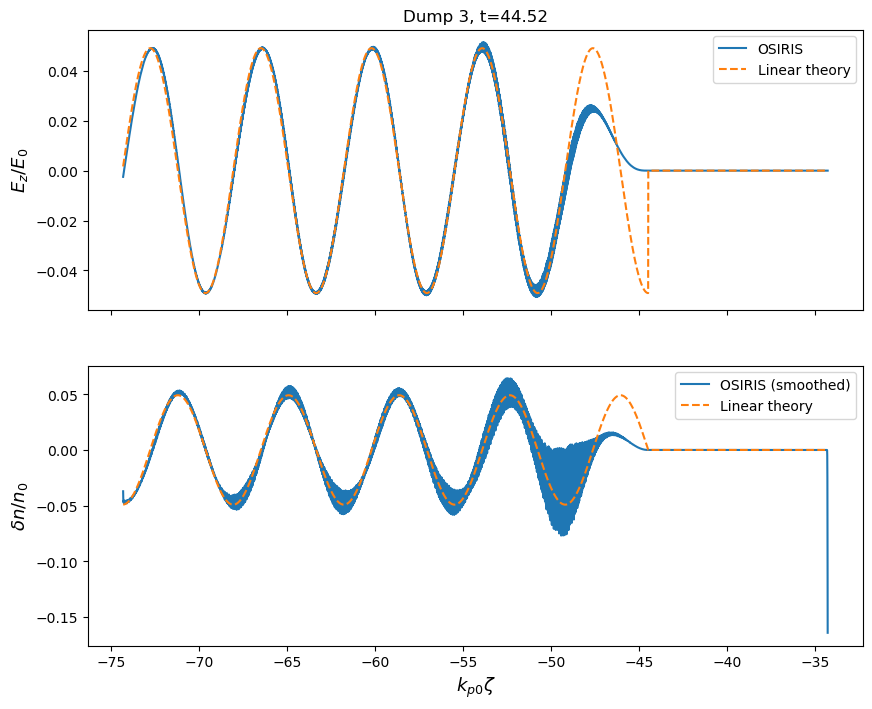
\includegraphics[width=\linewidth]{figures/validation-1D/dump3-linear.png}
        \caption{Dump 3}
        \label{fig:linear_1D_dump3}
    \end{subfigure}
    \hfill
    \begin{subfigure}{0.48\textwidth}
        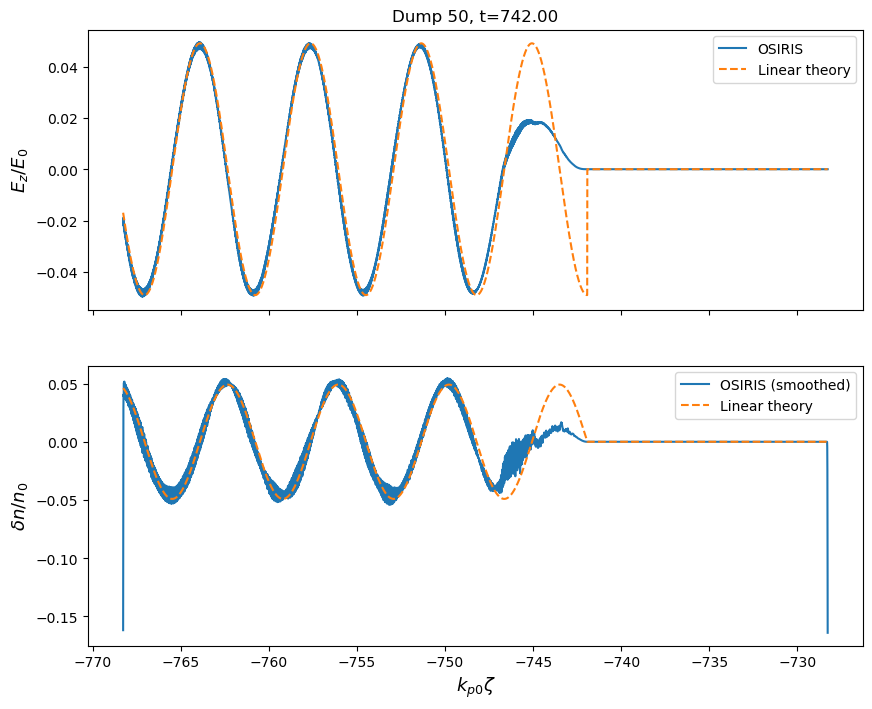
\includegraphics[width=\linewidth]{figures/validation-1D/dump50-linear.png}
        \caption{Dump 50}
        \label{fig:linear_1D_dump50}
    \end{subfigure}
    \caption{Comparison of simulated (OSIRIS) and analytic linear wake 
    solutions for a sine-squared pulse at two different dump times.
    Top: axial electric field $E_z/E_0$. Bottom: density perturbation
    $\delta n/n_0$.}
    \label{fig:linear_1D_sine}
    \end{figure}

    \subsubsection{Notes}

\subsection{Nonlinear Regime}
    
    Unlike the linear regime, the nonlinear regime doesn't ...

    \subsubsection{Derivation}

    Following Esarey et al. (2009), the 1D nonlinear wake potential
    $\phi$ satisfies
    \begin{equation}
        k_p^{-2}\frac{\partial^2\phi}{\partial\xi^2} = 
        \frac{1+a^2}{2(1+\phi)^2} - \frac{1}{2},
        \label{eq:nonlinear_wake}
    \end{equation}
    where $\gamma_\perp^2 = 1+a^2$ is the transverse quiver Lorentz factor
    of the plasma electrons. Unlike the linear case, this equation cannot
    be solved analytically in closed form for a general pulse profile, so
    it is instead integrated numerically as an initial value problem,
    starting from undisturbed plasma ahead of the pulse.


    For this regime, rather than analytically (mathematically) solving for
    the expressions of the wake, etc., we will just write a simple solver, 
    which we can test by trying to replicate the figure from the (BLANK) paper.

    \subsubsection{Solver Implementation}

    \begin{pythoncode}
    def solve_nonlinear_wake(a0, L_rms, k_p, k_pulse, zeta_range):

        # The analytic expression of the Gaussian profile we're using for the
        # photon distribution
        def a2(z):
            return a0**2 * np.exp(-z**2 / (2*L_rms**2)) * np.cos(k_pulse*z)**2

        # Make the second-order differential equation into a system of first
        # order differential equations
        def rhs(z, y):
            phi, dphi = y
            numerator = 1 + a2(z)
            d2phi = k_p**2 * (numerator / (2*(1+phi)**2) - 0.5)
            return [dphi, d2phi]

        # Initial conditions: phi = dphi/dzeta = 0 ahead of the pulse, where the
        # plasma is undisturbed
        y0 = [0.0, 0.0]

        # Evaluation grid for the returned solution
        zeta_eval = np.linspace(zeta_range[0], zeta_range[1], 10000)

        # Set a maximum step size so the fast oscillations can be resolved
        # (the cosine term in the above equation for a^2)
        max_step = (2*np.pi/k_pulse) / 20.0

        # Solve the system given all of this information
        sol = solve_ivp(rhs, [zeta_range[0], zeta_range[1]], y0, t_eval=zeta_eval, method='RK45', rtol=1e-8, atol=1e-10, max_step=max_step)

        zeta_sol = sol.t
        phi = sol.y[0]
        dphi = sol.y[1]
        numerator = 1 + a2(zeta_sol)

        # Ez/E0 = -dphi/dzeta (normalized axial field from the potential).
        Ez_E0 = -dphi

        # Nonlinear density perturbation
        n_n0 = (numerator + (1+phi)**2) / (2*(1+phi)**2)
        dn_n0 = n_n0 - 1.0

        return zeta_sol, Ez_E0, dn_n0, phi
    \end{pythoncode}

    Using this, we can replicate Figure 8 in the Esarey paper:
    
    \subsubsection{Gaussian Pulse : Setup}

        

    \subsubsection{Gaussian Pulse : Results}


    \subsubsection{Gaussian Pulse : Setup}


    \subsubsection{Gaussian Pulse : Results}




  \subsection{Comparison with Full EM Simulation}
    \subsubsection{zpulse Equivalent Setup}
    \subsubsection{Wake Amplitude Comparison}
    \subsubsection{Photon Phase Space Comparison}
  \subsection{Reproduction of Trines et al. 2007}
    \subsubsection{Parameters and Setup}
    \subsubsection{Results: Figure 2 Comparison}
    \subsubsection{Discussion and Discrepancies}

\newpage
\section{Validation: 2D Cartesian}


\newpage
\section{Validation: Quasi-3D / Cylindrical}

\subsection{Linear Regime}
    \subsubsection{Setup}
    \subsubsection{Results}
\subsection{Nonlinear Regime}
    \subsubsection{Setup}
    \subsubsection{Results}
\subsection{Comparison with Full EM Simulation}

\newpage
\section{Validation: 3D Cartesian}

\newpage
\section{Applications}

\subsection{Photon Acceleration in Plasma Wakefields}
\subsection{Raman Scattering}

\newpage
\section{Open Questions and Future Work}

\subsection{Unresolved Physics Questions}
\subsection{Planned Extensions}

% -- End of main content -------------------

% -- Start of appendices -------------------
% ------------------------------------------

\end{document}
